\documentclass[letterpaper]{article}

\usepackage{aaai}
\usepackage{times}
\usepackage{helvet}
\usepackage{courier}
\usepackage{url}
\usepackage{graphicx}
\usepackage{listings}
\usepackage{fancyvrb}
\frenchspacing

\title{Level Generator for \textit{Laserverse} using ASP}
\author{Abhijeet Krishnan \\ North Carolina State University \\ akrish13@ncsu.edu}
\date{December 2018}

\begin{document}

\maketitle

\begin{abstract}
    Procedural level generation is a great way to create more content and unexpected scenarios within a game
    \cite{gamasutra}. We demonstrate a level generator built for the puzzle game \textit{Laserverse} using Answer Set
    Programming (ASP). The design of the generator is explained and design decisions are justified. An evaluation of the
    generator is presented using playability as a metric. We discuss the challenges faced while writing the generator as
    well as possible avenues for improvement - both of the generator as well as the process of writing a generator using
    ASP.
\end{abstract}

\section{Introduction}
Procedurally generated levels are a major aspect of PCG research since they have the potential to allow almost any game
to be infinitely replayable. However, level design is a complex and creative discipline in which current procedural
level generators generally fail to match up to human level designers. Togelius et. al. \cite{togelius2013procedural}
describes some of the problems seen in generated levels for \textit{Super Mario Bros.}, namely a lack of progression and
macro-structure, a lack of storytelling or teaching, inexplicable structures and content, difficulty spikes and repeated
structures. While we recognized that the field is ripe for greater advancement, we settled on the modest goal of simply
designing a working generator for our game.

\textit{Laserverse} is a puzzle game developed in PuzzleScript by Martens et. al. \cite{laserverse} for the purpose of
studying the theory of mental model matching. The hypothesis of this work was that players learn puzzle game mechanics
through an iterative process of hypothesizing, failure and revision of mental models. The game was designed with a
number of mechanics designed to interact in a wide array of combinations. Our goal was to support this work by designing
a level generator which offered control over the specific mechanics used in the levels, enabling the authors to test
their hypothesis on a wider variety of participants without having to hand-author multiple levels.

We also present an evaluation of our generator using the metrics of \textit{playability} and \textit{solution length}.

\section{Background}

\subsection{Level Generation using ASP}
ASP is a programming paradigm (like procedural or functional programming) geared towards solving NP-hard search
problems. The problem domain is specified as a set of rules (or facts) and stable models are generated which satisfy all
those rules. If we can specify our game's level design space as a set of ASP constraints, we can use a solver to
generate solutions which satisfy those constraints, each of which is a playable level. We use clingo, part of the
Potassco answer set solving collection \cite{gebser2011potassco} as our solver of choice.

Smith and Mateas' paper \cite{smith2011answer} was the first one to argue in favour of ASP as a useful tool for
procedural content generation, citing ASP's brevity, expressiveness and generality in quickly constructing design spaces
for games. Later work by the authors on a puzzle game Refraction \cite{smith2012case} was also useful, since the game
shares some similarities with \textit{Laserverse}. A book chapter by the same authors \cite{nelson2016asp} provides more
instruction in how to write generators for mazes.

\subsection{\textit{Laserverse}}

\begin{figure}
    \centering
    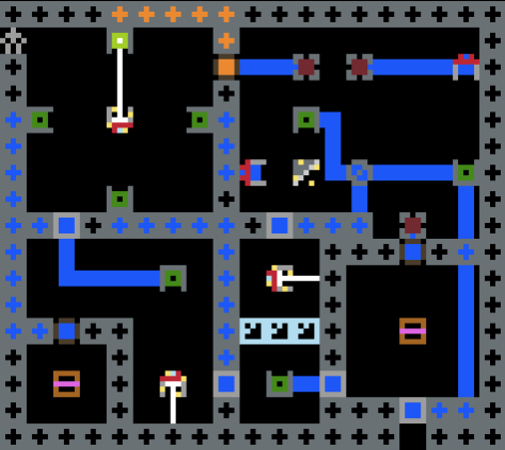
\includegraphics[width=0.47\textwidth]{img/wirefu.png}
    \caption{Screenshot of \textit{Laserverse} level \textit{Wire-fu} (hand-authored)}
    \label{fig:wirefu}
\end{figure}

\textit{Laserverse} is a puzzle game built using the PuzzleScript game engine \cite{puzzlescript}. It offers a simple
rule-based syntax for describing actions in the game world. For example, say we want the player to push a crate if the
player walks into it. We can express this succinctly in PuzzleScript as
\begin{Verbatim}[fontsize=\small]
[ > Player | Crate ] -> [ > Player | > Crate ]
\end{Verbatim}

\textit{Laserverse} is centered around the idea of interacting with lasers and mirrors in game to power sensors, which
then open doors to the exit. There are additional mechanics such as buttons, crates, splitters and logic gates. A full
explanation of each mechanic in the game can be found in the original paper, with mechanics missing from the original
paper described in Figure \ref{tab:mechanics}. The mechanics for \textit{Laserverse} are expressed in about $121$ lines
of PuzzleScript.

\begin{figure*}
    \centering
    \begin{tabular}{|l|l|}
        \hline
        Movable Laser      & Like the basic laser, but the player can move it around the game world without changing its
        orientation                                                                                                      \\
        \hline
        Movable Mirror     & Like the basic mirror, but the player can move around it the game world without changing
        its orientation                                                                                                  \\
        \hline
        Crate              & Can be moved around the game world and dropped onto buttons to keep them activated
        \\
        \hline
        Splitter           & Splits an incoming beam of light into two perpendicular beams
        \\
        \hline
        Rotatable Splitter & A splitter that the player can rotate to choose where the split beams are incident.
        \\
        \hline
        Movable Splitter   & Like the basic splitter, but the player can move it around the game world without changing
        its orientation                                                                                                  \\
        \hline
        AND Gate           & Activates only if both inputs are activated
        \\
        \hline
        Open Door          & A door which is open by default, and closes when activated
        \\
        \hline
        Glass Pane         & A transparent block which is solid but allows laser beams to pass through it
        \\
        \hline
        Sensor             & Activates a wire if a laser beam is incident on it
        \\
        \hline
        Guard              & Prevents a laser beam from striking a goal, usually allows beams from a single direction
        only                                                                                                             \\
        \hline
    \end{tabular}
    \caption{Elemental mechanics in \textit{Laserverse}}
    \label{tab:mechanics}
\end{figure*}

\subsection{Generator Evaluation}
The idea for evaluating the design space of a generator was first proposed in Smith and Whitehead's
\cite{Smith:2010:AER:1814256.1814260} seminal paper on the topic, in which they also presented an evaluation of a level
generator for their game \textit{Launchpad}. The idea is to define comparison metrics using which generated levels can
be compared. The metrics chosen should reflect global properties of levels and aid in understanding a generator's
expressive range. With these metrics, we can then visualize how the expressive range of a generator changes when
modifications are made to the generator.

For our generator, we define the comparison metrics of \textit{playability} and \textit{solution length}. Playability is
a boolean value which is True if the level is playable i.e. a solution exists, and False if it is not. Solution length
is a measure of the minimum number of steps required to solve a certain level.

\section{Approach}
Explain what you did in sufficient detail that someone could reproduce your work. High-level algorithm descriptions,
equations, and descriptions of your implementation decisions are all in-scope. Explain how you evaluated your work.

\subsection{Defining a design space}
The highly useful approach to defining the design space of all possible levels would be to restrict ourselves to
playable levels. This would require a notion of \textit{playability}. As will be described later, coming up with this
notion for a game like \textit{Laserverse}, with so many interacting mechanics, proved too difficult.

To simplify the design space, we opted to restrict ourselves to levels with a fixed kind of solution. We identified
three such solution types.
\begin{enumerate}
    \item Player picks up crate - player drops crate on button - button opens door to exit - player walks to exit
    \item Player rotates laser - laser activates sensor - sensor activates wires to door - door opens to exit - player
          walks to exit
    \item Player rotates laser - laser reflects off mirror - reflected beam activates sensor - sensor activates wires to
          door - door opens to exit
\end{enumerate}

This leads to a lot of simplifications. We only need one of each object for whichever level we generate (e.g. one
button, one crate and one door for level of type 1). We can define playability in terms of the existence of paths
between each objects in the solution. We can ignore all other mechanics and object types present in \textit{Laserverse}.

We follow the generate and test methodology to develop our generator. We generate all possible levels with the line -
\begin{Verbatim}[fontsize=\small]
{ at(X, Y, T) :tile(T) } = 1 :- dimX(X), dimY(Y).
\end{Verbatim}

This tries every possible tile (object) type for every possible tile location in the game. This is clearly just a brute
force enumeration of every possible level in the design space, so we refine this design space with additional rules.

We define cardinality constraints for each type of object in the game. This allows a designer to change the number of
these objects in generated levels. Given our design space, we would only get playable levels if we fix the number of
objects as $1$. The code for this can be seen below.

\begin{Verbatim}[fontsize=\small]
#const minLasers = 1.
#const maxLasers = 1.
minLasers { at(0..n-1, 0..m-1, T) :laser(T) }
    maxLasers.
\end{Verbatim}

We also constrain our levels to a $6 \times 6$ grid to reduce generation time. This can be modified, but generating a
level would take longer.

We add some rules to ensure our design space matches the authored levels. For example, we add rules to ensure that the
border is a wall and that the player and exit both lie on the border. To enforce playability, we require that the player
and exit not lie on a corner.

We then add rules specific to each level type. For example, in type 2, we add rules which prevent the laser from being
blocked by anything on its path to the sensor.

Now by enabling the rules for each level type in turn, we can generate levels of each type. These levels are not
guaranteed to be playable, since the paths to various objects might be blocked, and we have not added rules which
explicitly disallow this (due to the difficulty encountered when writing such rules).

\subsection{Evaluation}
The choice of suitable comparison metrics for puzzle games is an open question. One possible metric is the sense of
surprise experienced by players when they discover how mechanics interact in unexpected ways to lead to a solution, but
it is tricky to quantify this. In any case, we have very few mechanics we choose to work with for our evaluation, since
we want to have a large number of playable levels.

Therefore, we opt for the relatively simple metrics of playability and solution length to differentiate our levels. We
measure solution length only for playable levels. We have written a DFS-based agent in Python to solve our generated
levels to measure these metrics. The complete code for our generators and evaluators can be on found on
GitHub\footnote{\url{https://github.ncsu.edu/akrish13/laserverse-level-generator}}.

\section{Results}

\subsection{Playability}
\begin{figure}[h]
    \centering
    \begin{tabular}{|c|c|c|c|}
        \hline
               & Playable & Unplayable & Total  \\
        \hline
        Type 1 & $548$    & $452$      & $1000$ \\
        \hline
        Type 2 & $466$    & $534$      & $1000$ \\
        \hline
        Type 3 & $537$    & $463$      & $1000$ \\
        \hline
    \end{tabular}
    \caption{Number of playable levels for each level type}
    \label{tab:playable}
\end{figure}

\subsection{Solution Length}
\begin{figure}[h]
    \centering
    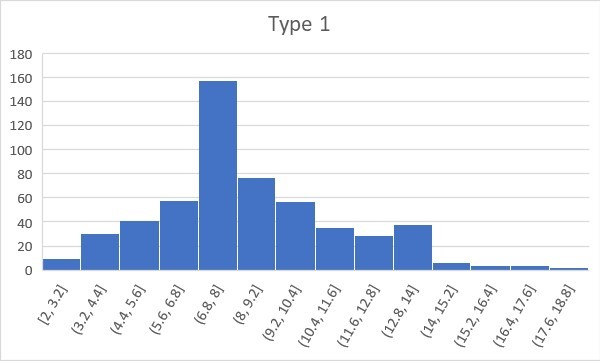
\includegraphics[width=0.4\textwidth]{img/crate.jpg}
    \caption{Histogram of solution lengths for type 1 level}
    \label{fig:crate}
\end{figure}

\begin{figure}[h]
    \centering
    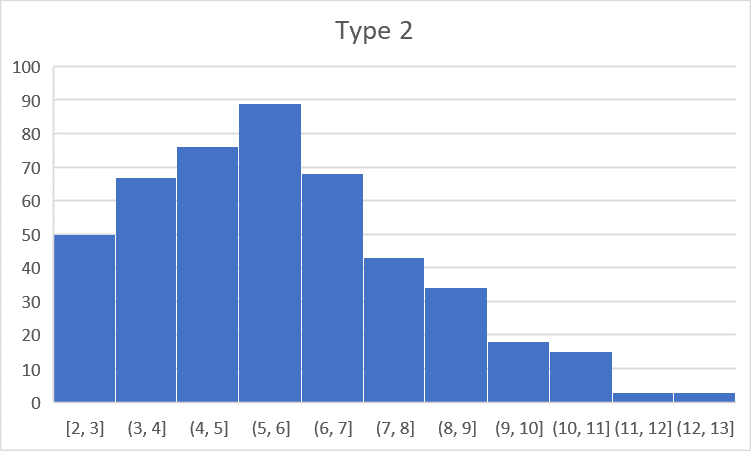
\includegraphics[width=0.4\textwidth]{img/laser.png}
    \caption{Histogram of solution lengths for type 2 level}
    \label{fig:laser}
\end{figure}

\begin{figure}[h]
    \centering
    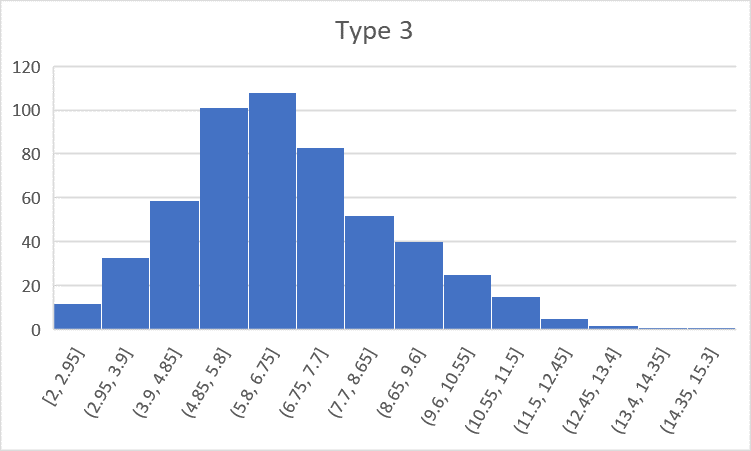
\includegraphics[width=0.4\textwidth]{img/mirror.png}
    \caption{Histogram of solution lengths for type 3 level}
    \label{fig:mirror}
\end{figure}

\section{Discussion}

\subsection{Challenges}

\subsubsection{Lack of expressivity}
A general notion of playability is hard to accurately capture for \textit{Laserverse}. We can look to another puzzle
game called Sokoban, which has also been implemented in PuzzleScript. A generator for Sokoban was implemented by the
team behind clingo for the $3^{rd}$ Answer Set Programming Competition \cite{aspcomp} using time as a variable to
represent a plan of actions. However, Sokoban has only a few actions, while \textit{Laserverse} has many, depending on
the objects in the environment. Therefore, a notion of playability would involve finding a plan of actions which would
solve a given level. This is difficult to code using ASP. Indeed, the simple notion of having a single wire connect two
objects was also difficult to conceptualize and code. This could be due to the author's inexperience with ASP.

\subsubsection{Lack of software engineering tools}
Common tools such as a debugger have no equivalent while working with ASP. Say a certain new rule is causing undesired
answer sets to be produced, or more commonly, causing the solver to return an UNSATISFIABLE verdict. It is difficult to
pinpoint why exactly this happens without a deep knowledge of ASP or logic programming. Tools which expose the inner
working of the solver better would be useful here. There has been some work on software engineering for ASP
\cite{febbraro2011aspide}, but there was no tool which proved useful to us.

Additionally, since the codebase for this generator was uncommonly large, it would be helpful to have a facility similar
to make for C/C++ programming which can utilize rules written in different files together. This would aid modularity and
ease while developing generators using ASP.

Levels generated using ASP also suffer from lack of intent and storytelling.

\subsection{Improvements and Future Work}
While additional and more complex level types can always be constructed, the ultimate goal would be to capture a general
notion of playability in ASP. The idea of using mission generation to generate a desired solution using ASP, and then
using ASP to embed that in a puzzle grid layout seems promising.

\bibliographystyle{aaai}
\bibliography{ref.bib}

\end{document}
